\section{Circuit série et intensité (4 points)}

\begin{questions}
	\question Trace le schéma normalisé du circuit ci-dessous. Repère les intensités $I_1$ à $I_4$ qui sont mesurées par les ampèremètres $A_1$ à $A_4$.
	
	\question L'ampèremètre $A_3$ mesure une intensité $I_3$ de \num{0.250} A. Que valent $I_1$, $I_2$ et $I_4$.
\end{questions}

\begin{center}
	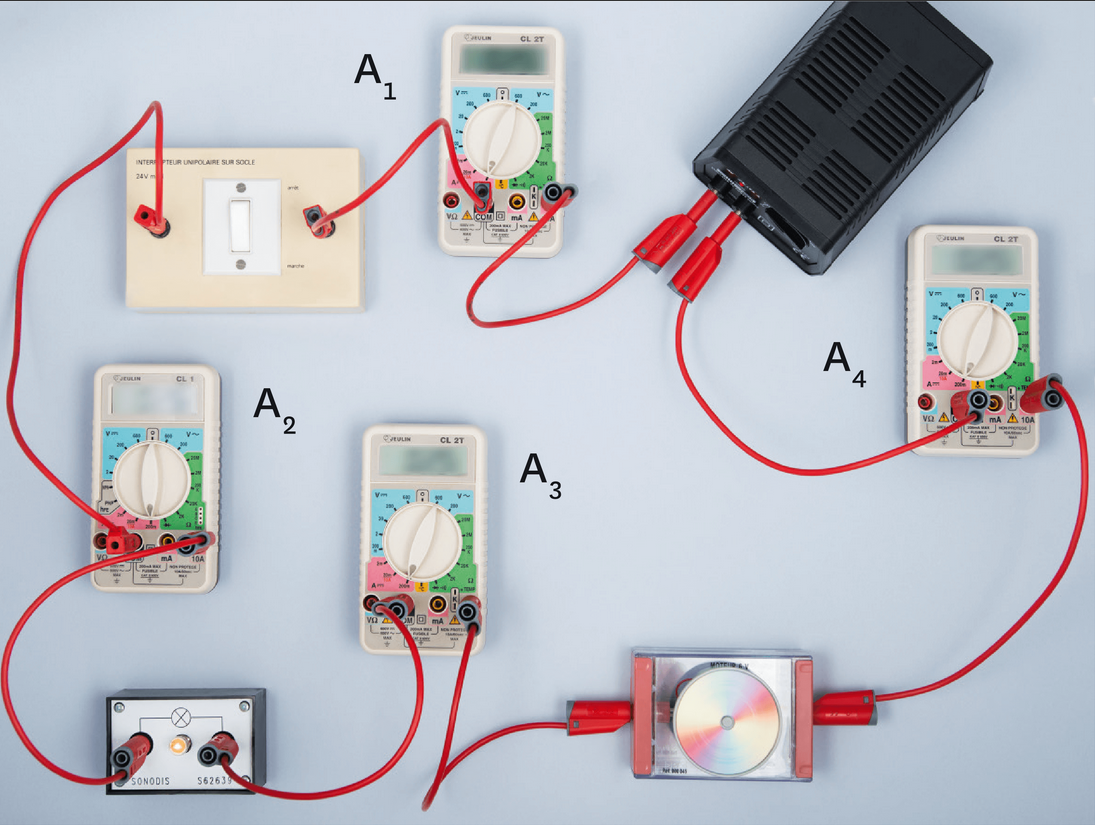
\includegraphics[scale=0.4]{img/ex15}
\end{center}